\subsection{HDF5}
HDF5 is a versatile data model containing complex data objects and metadata. 
Its information set is a collection of datasets, groups, datatypes and metadata objects. The data model defines mechanisms for creating associations between various information items. The main components of HDF5 are described below.

File:
In the HDF5 data model the container of an HDF5 infoset
is represented by a file. It is a collection of objects and also explains the relationship between them.
Every file begins with a root group "/", which serves as the "starting-point" in the object hierarchy. 

Dataset:
HDF5 datasets are objects that represent actual data or content. Datasets are arrays which can have multiple dimensions. A dataset is characterized by a dataspace and a datatype. The dataspace captures the rank (number of dimensions), and the current and maximum extent in each dimension. The datatype describes the type of its data elements. 

Group:
A group is an explicit association between HDF5 objects. It is synonymous with directories in a file system. A group could contain multiple other groups, datasets or datatypes \textit{within} it. 

Attribute:
Attributes are used for annotating datasets, groups, and datatype objects. They are datasets themselves, and are \textit{attached} to the existing objects they annotate. 

For example, as shown in figure~\ref{hdf5_example}, the file "Sample.h5" contains the root group which itself contains a group G1 and two datasets, D1 and D2. Group G1 contains a dataset D3. Attribute A1 is linked to dataset D1. The objects and the relationships between them can be represented as a B-tree, which is used internally by HDF5 to index its objects. 

\begin{figure}[!t]
\centering
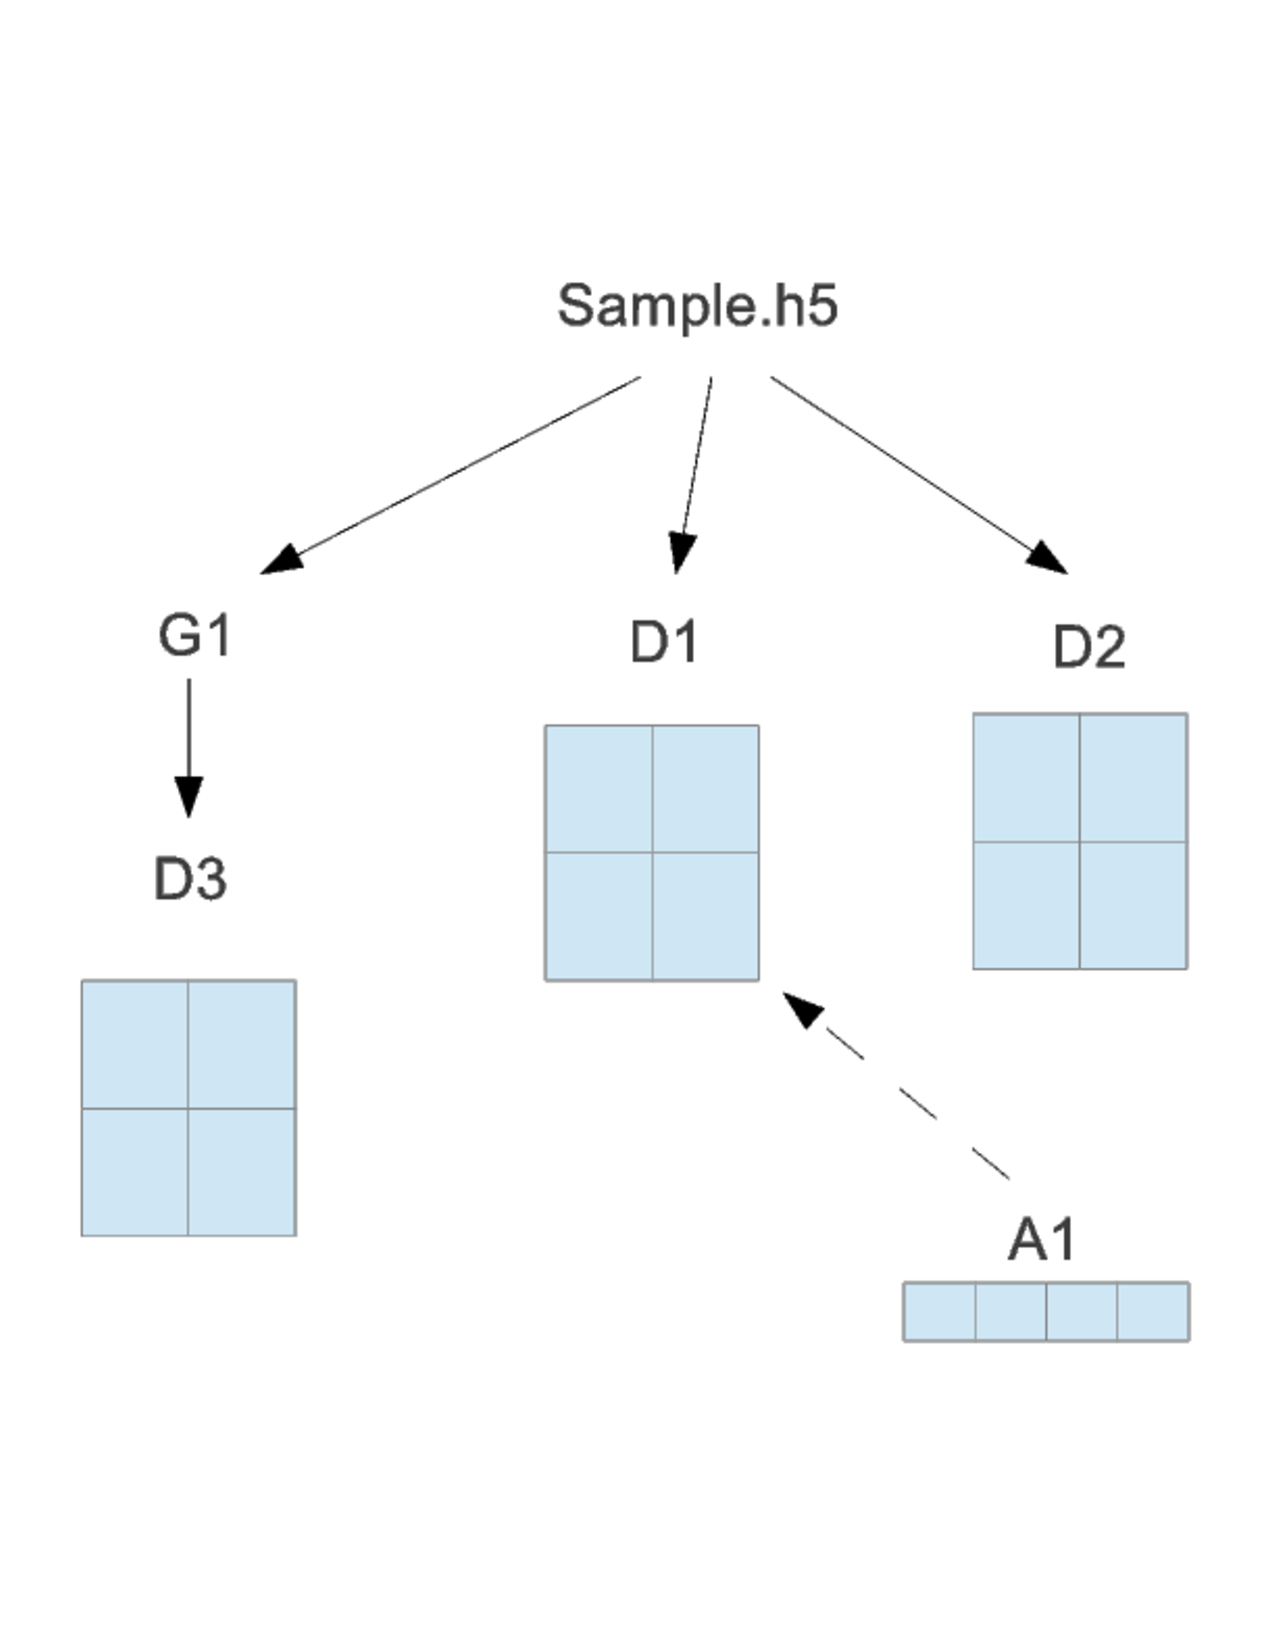
\includegraphics[width=2.5in]{hdf5_example}
\caption{A sample HDF5 file}
\label{hdf5_example}
\end{figure}

%Parallel HDF5 (PHDF5):
%HDF5 supports parallelism using MPI. Multiple processes can be used to access objects in a file. PHDF5 exports a parallel I/O interface, internally making use of MPI-IO. 
%Applications typically store multiple objects in a single HDF5 file. However, many popularly used parallel file systems like Lustre, Panasas etc. are known to perform poorly for workloads where multiple processes access a shared file. 

Virtual Object Layer (VOL):
The Virtual Object Layer (VOL) is a new abstraction layer internal to the HDF5 library~\cite{vol}. It is implemented just below the public API. The VOL exports an interface that allows writing plugins for HDF5, thereby enabling developers to store objects in a format different from the default HDF5 file format (like native netCDF or HDF4 format). Plugin writers provide an implementation for a set of functions that access data on disk. These include functions for file management, dataset creation and access, group creation, to name a few.

\subsection{PLFS}
PLFS is a middleware virtual file system that converts writes to a shared logical file into writes to multiple physical files. 
It is situated between the application and the parallel file system responsible for the actual data storage. 
It transforms N-1 into N-N, where every process participating in I/O writes data to its own, separate file. 
The basic operation of PLFS is as follows. For every writer to a logical file, PLFS creates a unique physical file on the underlying parallel file system. 
It also maintains sufficient metadata to recreate the shared logical file. 
We added a new feature to PLFS called extendible attributes (Xattrs). Xattrs serve as short, extensible metadata stored as key-value pairs.
They can be used to store user-defined information about data for easy and fast retrieval. 
%We use xattrs to store metadata about HDF5 datasets. For example, the datatype, number of dimensions and their extent are stored as xattrs. 

Users can interface with PLFS directly by using the PLFS API or by using an MPI library that has been integrated with PLFS (ad\_plfs layer).  




